\documentclass[aps, prc, reprint, amsmath, groupedaddress, nofootinbib]{revtex4-1}
%\usepackage[compat=1.1.0]{tikz-feynman}
\usepackage[utf8]{inputenc}
\usepackage{hyperref}
\usepackage{amsmath}
\usepackage{amssymb}
\usepackage{amsfonts}
\usepackage{tabularx}
\usepackage{booktabs}
\usepackage{graphicx}
\usepackage{color}
\usepackage{multirow}
\usepackage{verbatim}
\usepackage[inline]{enumitem}
\graphicspath{{fig/}}
\definecolor{theblue}{RGB}{0,50,230}
\usepackage{appendix}
\hypersetup{
  colorlinks=true,
  linkcolor=theblue,
  citecolor=theblue,
  urlcolor=theblue
} 
\usepackage[most]{tcolorbox}

\begin{abstract}
Highly energetic partons  created in perturbative processes at the onset of relativistic heavy-ion collisions  are excellent probes for the study of hot and dense deconfined QCD matter. This is accomplished by relating the energy-loss these partons suffer to the properties of the medium they traverse.
Monte-Carlo event generators, that allow for the realistic description of fluctuating initial conditions and medium properties, have become a powerful tool in this endeavor. However, the implementation of quantum coherence effects, such as the Landau-Pomeranchuk-Migdal (LPM) effect, poses a serious challenge to this class of models, since multiple interactions with the medium cannot be factorized into independent processes. 
In this work, we discuss several common implementations of the LPM effect in Monte-Carlo event generators and compare them to limiting cases in jet energy-loss theory for which semi-analytic calculations exist. We propose an approach, dubbed
``modified rescattering", that reproduces the limiting semi-analytic calculations of radiative parton energy loss for infinite and thin media  and reasonably describes gluon emission spectra. We study the impact of an expanding medium, a running coupling and heavy quark masses in this approach. 
\end{abstract}

\begin{document}
\title{Monte-Carlo Modeling of the Landau-Pomeranchuk-Migdal effect for Medium-induced QCD Splitting Processes}
\author{Weiyao Ke}
\author{Yingru Xu}
\author{Steffen A.\ Bass}
\affiliation{Department of Physics, Duke University, Durham, NC 27708-0305}
\date{\today}
\maketitle 

\section{Introduction}
The study of hard probes in relativistic heavy-ion collisions is moving towards the precision era thanks to upcoming experimental upgrades \cite{ATLAS-Collaboration:2012iwa,Abelevetal:2014dna,STAR:upgrade-hf,Adare:2015kwa,CMS:2017dec} as well as theoretical and computational advances that allow for the execution of jet energy-loss calculations in a realistic Quark-Gluon-Plasma (QGP) medium (including event-by-event fluctuating initial conditions and temperature-dependent transport coefficients) \cite{Wang:1994fx,Zakharov:1996fv,Baier:1996sk,Zakharov:1997uu,Arnold:2002zm,Gyulassy:2003mc,Kovner:2003zj,CasalderreySolana:2007pr,Bass:2008rv,Schenke:2009gb,Majumder:2009zu,Majumder:2010qh,Armesto:2011ht,Zapp:2011ya,Ovanesyan:2011xy,Kang:2014xsa,Cao:2016gvr,Kauder:2018cdt,Cao:2017zih}. Among the goals for this research is the characterization of the QGP medium in terms of its jet transport coefficients $\hat{q}$.

Monte-Carlo event generators are powerful tools that allow for the realistic description of fluctuating initial conditions and medium properties. 
However, the numerical implementation of quantum coherence effects, such as the Landau-Pomeranchuk-Migdal (LPM) effect, poses a serious challenge to this class of models, because coherent multiple interactions cannot be factorized into independent scatterings with the medium. 
In a dense medium, the LPM effect is important for the treatment of radiative energy-loss, which is the dominant contribution to energy-loss of partons traversing the QGP at high momentum.
Here, multiple scatterings during the gluon formation time act coherently to suppress the radiation spectrum \cite{PhysRev.103.1811,Wang:1994fx,Zakharov:1996fv,Zakharov:1997uu,Baier:1996kr,Baier:1996sk}.
Therefore, a medium induced radiation becomes effectively an $n$-body to $(n+1)$-body process that extends in space-time.
This feature is particularly difficult to accurately implement in a Monte-Carlo approach, where interactions are usually based on few-body processes that are local.
To simplify the problem while still retaining essential qualitative features such as the characteristic emission spectrum and path-length dependence of the energy loss, different methods have been used in numerical simulations \cite{Djordjevic:2008iz,Cao:2013ita,ColemanSmith:2012vr,Xu:2004mz,Zapp:2011ya,Gossiaux:2012cv,Park:thesis}.
In this work we compare three of the most common implementations based on different approximations of radiative processes to perturbative kinetic theory predictions in idealized limits \cite{Arnold:2002zm,Arnold:2008zu,Arnold:2009mr,Baier:1996kr,Baier:1998yf}. 
As we shall see, a modified approach based on the method of \cite{Zapp:2011ya} works remarkably well.
This method, referred to as the ``modified rescattering" approach, reproduces analytic calculations of energy loss as a function of coupling constant, temperature, parton energy and path length.
It also reasonably well describes the gluon radiation spectra in both static and expanding media.
We introduce parameters to control its finite- and infinite-size behaviors separately.
The parameters can be fine-tuned to match the theory or be calibrated to experimental data;
therefore, the performance of the theory can be measured quantitatively on the landscape of this parameter space in a future statistical analysis.

This paper is organized as follows. Section \ref{section:qual} reviews the qualitative spectrum of the medium induced radiation.
In Section \ref{section:MC}, three Monte Carlo implementations of radiative processes are discussed. 
Semi-analytic results to which the Monte Carlo simulations are compared are briefly summarized in Section \ref{section:Theo}.
Major results are shown in Section \ref{section:results}.
Finally, we discuss in Section \ref{section:disscuss} effects induced by the running of the coupling constant, the expanding medium and heavy quark masses (dead-cone effect) in the ``modified rescattering" implementation. We summarize in Section \ref{section:summary}.

\section{Transport approach in the incoherent limit}\label{section:MC}
In this section, we describe the Monte Carlo model in detail. The partonic processes are categorized into elastic (particle number conserving) and inelastic processes (particle number non-conserving). 
The inelastic processes are further divided into parton-splitting and parton-jointing contribution. 
As a remark at the beginning, the QCD analog of the Landau-Pomeranchuk-Migdal (LPM) effect introduces coherence of medium-induce high energy splitting in dense QCD medium over a long distance, breaking the assumption of Boltzmann equation that interacts are treated as local in space-time.
In this section, we shall first proceed using local and incoherent calculation of such processes and will discuss in great detail in the next section on including the LPM effect in a Boltzmann-like transport approach.

The elastic interaction between hard parton and medium is separate into a large-momentum transfer (hard) and a small-momentum transfer (soft) part.
The switching scale is chosen to be proportional to the Debye mass square $Q_{\textrm{cut}}^2 = c m_D^2$, where $c$ is a parameter.
Respectively, the inelastic processes are also separated into diffusion-induced slitting / jointing processes, and large-$Q$ matrix-element based inelastic scattering contribution.

The large-$Q$ collisions are solved by a linearized Boltzmann equation with using collision rates calculated with vacuum matrix-elements, while the soft interactions are approximated by a diffusion process and is solved by Langevin equations.
This combined Langevin and linearized Boltzmann dyanmics is solved on the particle level using a two step approach,
\begin{eqnarray}
\vec{x}(t+\Delta t) &=& \frac{\vec{p}}{E}\Delta t\\
\vec{p}_{\textrm{int}} &=& \vec{p} - \eta_D \vec{p} \Delta t + \vec{\xi}(t) \Delta t\\
\Delta t\frac{dR(T, \vec{v}, \vec{p}_{\textrm{int}})}{d\vec{p}^3} &\xrightarrow{\textrm{sampling}}& \vec{p}(t+\Delta t)
\end{eqnarray}
Where the particle first does free transport, and then its momentum be updated with diffusion dynamics to get an intermediate $\vec{p}_{\textrm{int}}$. 
Then, the particle under goes collision according to the reaction probability within $\Delta t$, and the final states are obtained by sampling the differential collision rate.
The diffusion dynamics consists of a thermal random force such that,
\begin{eqnarray}
\left\langle\xi_i(t)\xi_j(0)\right\rangle = \delta(t) \left(
\frac{p_i p_j}{p^2}\hat{q}_{S, L} + \left(
\delta_{ij}-\frac{p_i p_j}{p^2}
\right)\frac{\hat{q}_S}{2} 
\right)
\end{eqnarray}
Because we require that the diffusion dynamics only accounts for soft momentum transfer processes, its transport coefficient is obtained by integrating the leading order collision kernel upto the momentum $Q_{\textrm{cut}}$,
\begin{eqnarray}
\hat{q}_S = \int dq^2 \frac{\alpha_s m_D^2 T}{q^2 (q^2+m_D^2)} \\
\hat{q}_{S,L} = \int dq^2 \frac{\alpha_s m_\infty^2 T}{q^2 (q^2+m_\infty^2)}
\end{eqnarray}
with the drag coefficient determined by the Einstein relation,
\begin{eqnarray}
\eta_D = \frac{\hat{q}_{S,L}}{2ET} - \frac{d\hat{q}_{S,L}}{dp^2} - \frac{2\hat{q}_{S,L} - 2\hat{q}_S}{2p^2}
\end{eqnarray}
For the large-$Q$ scattering processes, the collision rates for the $2\rightarrow 2$ and $2\rightarrow 3$ scatterings are obtained by integrating the vacuum matrix-element,
\begin{eqnarray}
R = \frac{d}{2E_1}\int  \frac{d^3p_2}{2E_2(2\pi)^3} f_0(p_2)2\hat{s} \int_{-\hat{s}}^{Q_{\textrm{cut}^2}}\frac{d\sigma}{d\hat{t}}d\hat{t}
\end{eqnarray}
The integration is restricted to large momentum transfer above $Q_{\textrm{cut}}$ and therefore we do not impose additional screening effect to regulate the matrix-element.
For the incoherent diffusion-induced splitting rate, we borrow the expression from [] stripping its time-dependent phase factor,
\begin{eqnarray}
R = \int d k_\perp^2 dx \frac{\alpha_s P(x) \hat{q}^S}{2\pi (k_\perp^2 + m_\infty^2)^2}
\end{eqnarray}
where a gluon thermal mass is added to screen the divergence.
For the reverse processes $3\rightarrow 2$  and $2\rightarrow 1$ processes, similar reaction rate can be written down.

The vacuum matrix-element is used for the large-$Q$ elastic and inelastic scatterings.
In this work, the $2\rightarrow 2$ matrix-element only includes the $\hat{t}$-channel contribution.
Regarding the $2\rightarrow 3$ matrix-element, in previous study [], we used to employ an improved version of the original Gunion-Bertsch cross-section that works under the limits $k_\perp, q_\perp \ll \sqrt{s}$ and $x q_\perp \ll k_\perp$.
In the present study, we keep improving the matrix-elements by following the derivation in in [] while relaxing the condition $x q_\perp \ll k_\perp$.
Therefore the updated matrix-elements contain the correct vacuum splitting function in the collinear limit.
We summarize the matrix-elements here and have attached a derivation in the appendix,
\begin{eqnarray}
\overline{|M^2|}_{g+q\rightarrow g+g+q} &=& \overline{|M^2|}_{g+q\rightarrow g+q} x(1-x) P_1\\
\overline{|M^2|}_{g+g\rightarrow g+g+g} &=& \overline{|M^2|}_{g+g\rightarrow g+g} x(1-x) P_1\\
P_1 &=& g^2  C_A\frac{1+x^4+(1-x)^4}{x(1-x)}   \\\nonumber
&\times&\left(\vec{A}^2 + \vec{B}^2 - \vec{A}\cdot\vec{B}\right)\\
\vec{A} &=& \frac{\vec{k}_\perp - x\vec{q}_\perp}{(\vec{k}_\perp - x\vec{q}_\perp)^2} -  \frac{\vec{k}_\perp - \vec{q}_\perp}{(\vec{k}_\perp - \vec{q}_\perp)^2} \\
\vec{B} &=& \frac{\vec{k}_\perp - x\vec{q}_\perp}{(\vec{k}_\perp - x\vec{q}_\perp)^2} -  \frac{\vec{k}_\perp}{\vec{k}_\perp^2}
\end{eqnarray}
for gluon splitting into two gluons. And for quark radiating a gluon, we have
\begin{eqnarray}
\overline{|M^2|}_{q+q\rightarrow q+q+g} &=& \overline{|M^2|}_{q+q\rightarrow q+q} x(1-x) P_2\\
\overline{|M^2|}_{q+g\rightarrow q+g+g} &=& \overline{|M^2|}_{q+g\rightarrow q+g} x(1-x) P_2\\
P_2 &=& g^2 C_F\frac{1+(1-x)^2}{x}  \\\nonumber
&\times&\left(\vec{A}^2 + \vec{B}^2 - \left(2-\frac{C_A}{C_F}\right)\vec{A}\cdot\vec{B}\right)\\
\vec{A} &=& \frac{\vec{k}_\perp - \vec{q}_\perp}{(\vec{k}_\perp - \vec{q}_\perp)^2} -  \frac{\vec{k}_\perp - x\vec{q}_\perp}{(\vec{k}_\perp - x\vec{q}_\perp)^2} \\
\vec{B} &=& \frac{\vec{k}_\perp - \vec{q}_\perp}{(\vec{k}_\perp - \vec{q}_\perp)^2} -  \frac{\vec{k}_\perp}{\vec{k}_\perp^2}
\end{eqnarray}
and finally for gluon splits into the quark-antiquark pair,
\begin{eqnarray}
\overline{|M^2|}_{g+q\rightarrow q+\bar{q}+q} &=& \overline{|M^2|}_{g+q\rightarrow g+q} x(1-x) P_3\\
\overline{|M^2|}_{g+g\rightarrow q+\bar{q}+g} &=& \overline{|M^2|}_{g+g\rightarrow g+g} x(1-x) P_3\\
P_3 &=& g^2 \frac{n_f C_F^2 d_F}{2C_A d_A}(x^2+(1-x)^2) \\\nonumber
&\times&\left(\vec{A}^2 + \vec{B}^2 - \left(2- \frac{C_A}{C_F}\right)\vec{A}\cdot\vec{B}\right)\\
\vec{A} &=& \frac{\vec{k}_\perp - x\vec{q}_\perp}{(\vec{k}_\perp - x\vec{q}_\perp)^2} -  \frac{\vec{k}_\perp - \vec{q}_\perp}{(\vec{k}_\perp - \vec{q}_\perp)^2} \\
\vec{B} &=& \frac{\vec{k}_\perp - x\vec{q}_\perp}{(\vec{k}_\perp - x\vec{q}_\perp)^2} -  \frac{\vec{k}_\perp}{\vec{k}_\perp^2}.
\end{eqnarray}
Here, the two body matrix-elements that enters the $2\rightarrow 3$ matrix-element is always required to be the $t$-channel contribution.

Combining all these processes, we summarize our linearized-Boltzmann plus Langevin equation into,
\begin{eqnarray}
\frac{df}{dt} = \mathcal{D}[f] + \mathcal{C}_{1\leftrightarrow 2}[f] + \mathcal{C}_{2\leftrightarrow 2}[f] + \mathcal{C}_{2\leftrightarrow 3}[f].
\end{eqnarray}
The distribution function of the hard parton under goes soft diffusion and diffusion induced-radiation. 
Hard collision with the medium are included as $2\leftrightarrow 2$ and $2\leftrightarrow 3$ collision terms.
The next section devotes to the inclusion of LPM effect to such an incoherent transport equation.

\section{Modeling LPM effect with histroy dependent transport approach}\label{section:modified-Boltzmann}
The LPM effects comes from that the parton splitting is not instantaneous but expend for a finite space-time, known as the formation time $\tau_f$ for a specific transition.
From uncertainty principal, the formation time can be obtained as the inverse of the difference between the final-state energy and the initial-state energy of the splitting,
\begin{eqnarray}
\tau_f^{-1} \sim \delta E = \frac{[(1-x)\vec{k}_\perp - x\vec{q}_\perp]^2}{2x(1-x)E} 
\label{eq:tauf}
\end{eqnarray}
In the reference frame where the initial parton moves in the $z$-direction, the formation time becomes $\tau_f = 2x(1-x)E/k_\perp^2$.
For high energy splitting, such a formation time can be very large compared to the mean-free-path $\lambda \sim 1/g^2T$ from leading order estimation.
During such time, the transfer momentum of the final states are also broadened due to these multiple scatterings, and in the diffusion limit one gets that on average
\begin{eqnarray}
\left\langle k_\perp^2 \right\rangle \approx \hat{q} \tau_f \label{eq:broaden}
\end{eqnarray}
Where $\hat{q} = d \left\langle k_\perp^2 \right\rangle / dt$ is the transverse momentum broadening parameter.
Combining Eq. \ref{eq:tauf} and Eq. \ref{eq:broaden}, a crude estimate for the average formation time is then $\left\langle \tau_f \right\rangle \sim \sqrt{\omega/\hat{q}}$.
The quantum nature requires that the multiple interactions within the formation time has to be resumed to contribute coherently to the transition rate.
In the large-medium limit, the leading effect is that the transition rate from interacting with $N$-scattering centers are reduced to the rate induced by interacting with an effectively $N\lambda/\tau_f$ coherent scattering centers. 
This reduction of radiation rate is the LPM suppression and in this large medium limit, the estimated suppression factor $\lambda/\tau_f \sim \sqrt{T/\omega}$ modifies radiation spectrum qualitatively at leading order when $\omega \gg T$.
Therefore, it is important for the transport model to reproduce such leading order features if one perform phenomenological study using high transverse momentum data obtained in the nuclear collisions.

The difficulty one encounters when attempting to include the LPM effect in the Boltzmann approach is that such semi-classical transport assumes local interaction.
The interactions are treated as point like scatterings in space-time, which is a good approximation for elastic processes at weak coupling $\lambda \gg 1/m_D$, but breaks down for high energy splitting where $\lambda \ll \tau_f$.
Certainly, quite fundamental modification has to be made to the Boltzmann equation to include splitting processes properly which we shall refers to as the history dependence.

In this section, we would like to show the approximation that we made to include the LPM effect into a Boltzmann-like transport approach.
The leading-order calculation of parton radiative energy-loss in a ``brick" medium and the comparison between different approximations has been discussed in detail in \cite{CaronHuot:2010bp}.
Here we quote their reorganized formula for medium-induced splitting,
\begin{eqnarray}
\frac{dP^{a}_{bc}}{d\omega} &=& \int_0^\infty dt \frac{g^2}{\pi E} P_{bc}^{a(0)}(x) \int_t^\infty dt'  F(t', t)\label{eq:LO-eq}\\
F(t', t) &=& \mathfrak{Re} \int_{{\bf q}', {\bf q}} \frac{i {\bf q}'\cdot {\bf q}}{\delta E} \mathcal{C}(t') K(t', {\bf q}'; t, {\bf q})
\end{eqnarray}
Where $P_{bc}^{a(0)}$ is the vacuum splitting function, $\delta E$ the energy difference between initial and final states. $\mathcal{C}(t')$ is a Boltzmann-like collision operator such that,
\begin{eqnarray}
\mathcal{C}[f] = \int_{\bf q} \frac{g^2 m_D^2 T}{q^2\left(m_D^2+q^2\right)}
&&\left\{  \frac{C_b+C_c-C_a}{2}\left(f_{\bf p}-f_{{\bf p}-{\bf q}}\right) \right.\\\nonumber
 +&&    \frac{C_a+C_c-C_b}{2}\left(f_{\bf p}-f_{{\bf p}+x{\bf q}}\right) \\\nonumber
+&&  \left. \frac{C_a+C_b-C_c}{2}\left(f_{\bf p}-f_{{\bf p}+(1-x){\bf q}}\right)\right\}
\end{eqnarray}
Where $C_i$ are the color factors of each parton.
Finally, $K$ is the quantum mechanical propagator of the Hamiltonian $\hat{H} = \delta E - i\mathcal{C}$ in the momentum representation.
This rather compact equation for leading order calculation is actually hard to implemented in a Monte Carlo way, due to the double time integral that signature the quantum nature of this transition.
Also, the solution for the propagator generally dependents on the temperature profile of such a brick medium, making it an increasingly difficult task for simulation in phenomenological situations like event-by-event fluctuating QGP evolutions.

\subsection{Ansatz for modifying the Boltzmann transport}
Our approximation towards a Boltzmann-like transport equation starts from replacing the time propagator $F(t',t)$ by a very simple ansatz,
\begin{eqnarray}
\int dt' F(t', t) \rightarrow \int dt' \frac{b}{\tau_f^2}\Theta(t'-t-a\tau_f).
\end{eqnarray}
This approximation is indeed very crude, but contains the qualitative behavior given that $\tau_f$ is a characteristic scale of the problem.
The prefactor $b/\tau_f^2$ takes care of the dimension of $F$ and the $\Theta$-function cut off the propagator beyond $\Delta t = t'-t > a\tau_f$, representing the finite time interval for coherent multiple interaction. 
Finally, $a$ and $b$ are dimensionless number whose form shall be discussed in detail in the next section and will be tuned to achieve an optimal level of agreement with the theoretical calculation.

With this is simple ansatz, the medium induced splitting probability becomes,
\begin{eqnarray}
\frac{dP^{a}_{bc}}{d\omega} &=& \int_0^\infty dt \frac{g^2 P_{bc}^{a(0)}}{\pi E\tilde{\lambda}(t)} \int_t^\infty dt'  \Theta(t'-t-a\tau_f) \frac{b \tilde{\lambda}(t)}{\tau_f^2} \\
&=& \int_0^\infty dt \frac{dR_{\textrm{incoh}}(t)}{d\omega} \times \left.\frac{ab\tilde{\lambda}(t)}{\tau_f(t',t)}\right|_{t'=t+a\tau_f}
\end{eqnarray}
where we have divided and multiplied back an effective mean-free-path $\tilde{\lambda}$ so that we interpret the quantity immediately after the $dt$ integral as an incoherent splitting rate $R_{\textrm{incoh}}$.
Now it becomes clear how one can modify the standard Botlzmann transport to include the LPM effect for the splitting process:
\begin{enumerate}
\item Evolve each particle by solving the collision rate equation with incoherent splitting rate at time $t$.
\item The daughter partons are not immediately treated as independent object, and is evolved together with the mother parton. Only elastic collisions are allowed for daughter partons (the mother parton can keep splitting).
\item Evolving the mother and preformed-daughter partons and recalculate the formation time until $t'-t > a\tau_f$ is satisfied.
\item At this point $t'$, reject this splitting process with probability $1-\frac{ab\tilde{\lambda}(t)}{\tau_f}$. Daughter partons from those accepted processes will be treated as independent objects from time $t'$ and will interact through both elastic and inelastic channels.
\end{enumerate} 
The key in such a procedure is a self-consistent determination of the formation time as described in step 3, which results in the expected scaling of the average formation time in the large static medium $\left\langle\tau_f\right\rangle \propto \sqrt{\omega/\hat{q}}$ and generalizes to medium with more complex temperature profile.
This iterative procedure was first developed and implemented by [].

\subsection{Matching the ansatz to semi-analytic calculation}
Such an ansatz only captures the qualitative behavior of the LPM effect in a large medium. 
To make it more useful, we try to match it to semi-analytic calculation of the underlying theory performed in an infinite medium.

In an infinite static medium, the formula for the gluon radiation spectrum (we only use the one for a gluon splitting from a quark) is derived in \cite{Arnold:2002zm,Arnold:2003zc},
\begin{eqnarray}\label{eq:AMY-1}
\nonumber
\frac{dP_{a\rightarrow bc}}{dt dx} &=& \frac{1}{2E\nu_a} \frac{\alpha_s d_a P_{a\rightarrow bc}(x)}{2x^2(1-x)^2}\int\frac{d^2\vec{h}}{(2\pi)^2}2\vec{h}\cdot \mathfrak{Re} \vec{F}
\end{eqnarray}
where we have dropped the Bose enhancement and the Pauli blocking factors from the original formula.
$\vec{F}(\vec{h}; p, x)$ satisfies the following equation,
\begin{eqnarray}\label{eq:AMY-2}
\nonumber
2\vec{h} &=& i\frac{h^2 \vec{F}(\vec{h})}{p^3 2x(1-x)} + g^2 \mathcal{C}[\vec{F}]
\end{eqnarray} 
The exact solution was solved numerically [], but we shall analyze using a semi-analytic solution to the next-to-leading-log accuracy obtained by the author of \cite{Arnold:2008zu}.
In their derivation at the leading log level, a momentum transfer scale $Q_0$ is introduced to the collision kernel $\mathcal{C}$ and a small-$q$ expansion is performed to obtained a diffusion approximation to $\mathcal{C}$ and is valid upto $Q_0$.
The resulting leading-log solution is,
\begin{eqnarray}\label{eq:AMY-LL}
\frac{dP_{a\rightarrow bc}^{\textrm{LL}}}{dt dx} &=& \frac{\alpha_s P_{a\rightarrow bc}(x)}{\pi}\frac{\sqrt{2}}{2}
\left(\frac{\hat{q}_3(x, Q_0^2)}{2x(1-x)E}\right)^{\frac{1}{2}}\\
\hat{q}_3(x, Q_0^2) &=& \alpha_s T m_D^2 \ln\left(1+\frac{Q_0^2}{m_D^2}\right) C_{abc}(x)\\
C_{abc}(x) &=&  \left(\frac{C_b+C_c-C_a}{2} + x^2 \frac{C_a+C_c-C_b}{2} \right.\\
&+& \left.(1-x)^2\frac{C_a+C_b-C_c}{2}\right)
\end{eqnarray}
Where the $\hat{q}_3$ is as an effective diffusion constant for conveniences. 
Comparing the leading-log formula to the simple ansatz we introduced to the modified Boltzmann approach, there is indeed a piece that playes the row of inverse formation time $\sqrt{\hat{q}_3 / 2x(1-x)E}$. However, the difference is that the effective $\hat{q}_3$ is different from the transport coefficient expected from the implemented gluon elastic re-scatterings by the $x$-dependent of the color factor combination $C_{abc}$.
This can be improved in the modified by making the $a$ parameter an color- and $x$-dependent quantity,
\begin{eqnarray}
a \rightarrow a_{abc}(x) = \frac{C_A}{C_{abc}(x)}
\end{eqnarray}
Because the leading-log approximation is only made with a upper bound for the momentum transfer,$\hat{q}_3$ has a logarithmic dependence on $Q_0^2$ that comes from integrating the collision kernel upto $Q_0$.
This unknown $Q_0$ parameter also introduces a large uncertainty to the lead-log formula.
In our Monte-Carlo simulation, the large-$Q$ matrix-element are always integrated upto the largest possible momentum transfer which is the center of mass energy $\hat{s}$.
In a thermal medium, the average of $Q_0^2$ or $\hat{s}$ will be $6ET$.

The problem of the undetermined $Q_0$ scale can be improved by going to the next-to-lead-log order, where the part of the collision kernel above $Q_0$ is treated as a pertrubation on top of the leading-log solution.
This single-hard correction to the multiple-soft calculation is also recently studied by the author of [] in the BDMPS framework.
In both works, a reasonable value of $Q_0$ can be determined at NLL order or self consistently in [], and the NLL spectrum looks like the LL solution but with $Q_0$ replaced by the $Q_{0}^{\textrm{NLL}}$,
\begin{eqnarray}
\frac{Q_{0}^{\textrm{NLL},2}}{m_D^2} \approx \frac{\sqrt{\omega \hat{q}(Q_0)}}{m_D^2} \approx \frac{\tau_f \hat{q}}{m_D^2} = \frac{\tau_f}{\tilde{\lambda}}
\end{eqnarray}
where in the last step, we express this quantity with the formation time and effective mean-free-path that is used in our modified Boltzmann approach.
Therefore, we can correct for the $Q$ scale in our approach by improving the $b$ parameter to 
\begin{eqnarray}
b = 0.75\sqrt{\frac{\ln\left(1+\tau_f/\tilde{\lambda}\right)}{\ln\left(1+6ET/m_D^2\right)}},
\end{eqnarray}
which corrects the na\"ive choice of $Q_0 \sim \sqrt{6ET}$ in the incoherent matrix-element integration.
The prefactor $0.75$ was tuned when comparing with our modified-Boltzmann simulation to the semi-analytic results in the next section, and will be the same for the rest of the paper.
This logarithmic correction comes from the $\sim 1/q^4$ perturbative tail of the collision kernel.
Therefore, if one implements anther collision kernel that vanishes exponentially at large-$q$, this logarithm factor in $b$ is unnecessary. 


\section{results}\label{section:results}
\begin{figure}
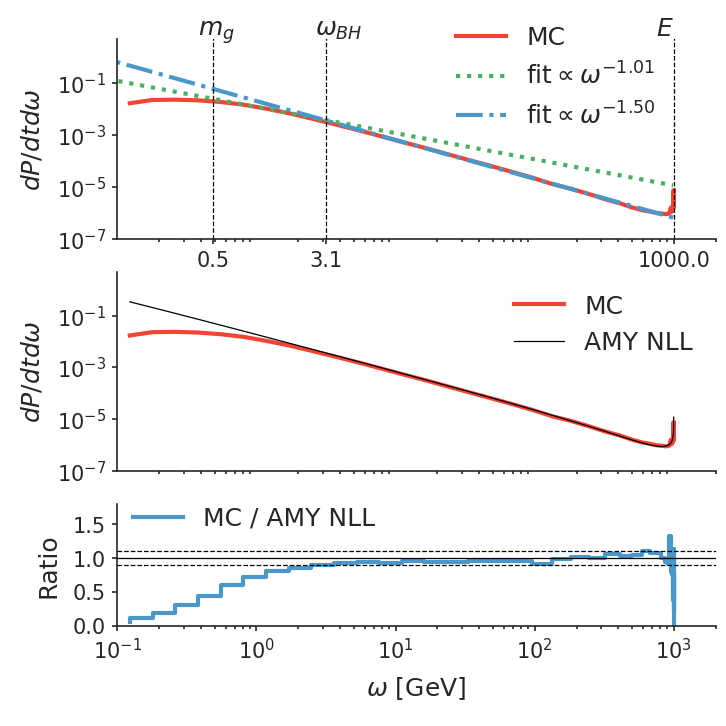
\includegraphics[width=\columnwidth]{spectrum.png}
\caption{Radiated gluon spectrum in an infinite medium from a quark of energy $E=q$ TeV, with a coupling constant $\alpha_s = 0.1$. The top frame shows the spectrum (red-dashed line) and power law fit (green-dotted and blue-dash-dotted lines) in different gluon energy ($0<\omega < E$) regions, separated by energy scales $m_\infty$, $\hat{q}_0\lambda_g^2 \sim 2\pi T$. The middle frame is the same calculation compared to the incoherent spectrum and the AMY semi-analytic result. The bottom frame is the ratio between the Monte-Carlo simulation and the semi-analytic calculation.}
\label{fig:spectrum}
\end{figure}
\begin{figure}
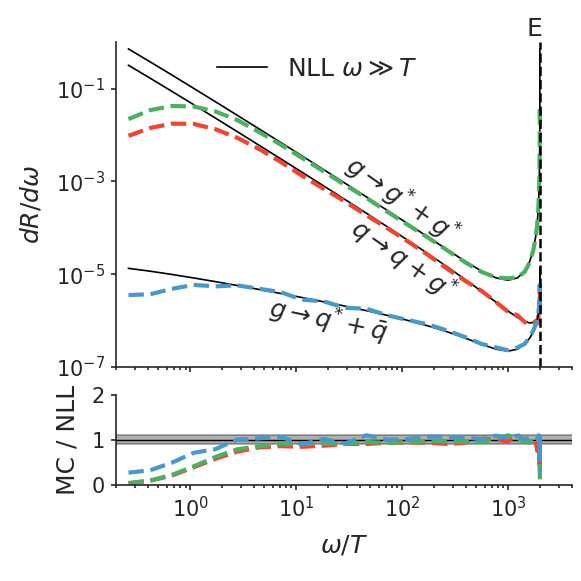
\includegraphics[width=\columnwidth]{channel_rate.png}
\caption{Radiated gluon spectrum in an infinite medium from a quark of energy $E=q$ TeV, with a coupling constant $\alpha_s = 0.1$. The top frame shows the spectrum (red-dashed line) and power law fit (green-dotted and blue-dash-dotted lines) in different gluon energy ($0<\omega < E$) regions, separated by energy scales $m_\infty$, $\hat{q}_0\lambda_g^2 \sim 2\pi T$. The middle frame is the same calculation compared to the incoherent spectrum and the AMY semi-analytic result. The bottom frame is the ratio between the Monte-Carlo simulation and the semi-analytic calculation.}
\label{fig:spectrum}
\end{figure}
In this section, we compare the splitting rate $dR/d\omega$ that comes out of the modified Boltzmann approach simulation to the NLL approximation in the infinite medium limit.


The differential rate in an infinite medium $dR/d\omega$ is shown in Figure \ref{fig:spectrum} for a 1 TeV quark.
Please also refer to Appendix \ref{app:tune-spectrum} for a full comparison varying both the parton energy and the coupling constant.
The upper figure shows different domains of the emission spectrum separated by the gluon thermal mass $m_\infty$ and an estimate of the Bethe-Heitler energy $\lambda_g m_D^2 \sim 2\pi T$.
We have chosen $\alpha_s = 0.1$ so that the separation between $m_\infty$ and $2\pi T$ is more visible.
The spectrum with $\omega < m_\infty$ is suppressed due the use of a finite mass.
In the Bethe-Heitler region $m_\infty < \omega < 2\pi T$, incoherent $2\rightarrow 3$ processes described in Equation \ref{eq:GB-rate} dominate and the spectrum scales like $\omega^{-1}$.
In the LPM region $2\pi T < \omega < E$, the spectrum is dominated by coherent multiple scatterings and should be proportional to $\omega^{-3/2}$.
The power-law fits in each domain are very close to the expected scaling.
In the middle figure, we compare the above Monte-Carlo implementation to a calculation using the incoherent rate and to the AMY NLL approximation and the ratio is shown in the bottom plot.
There is a good agreement of $dR/d\omega$ between the modified Boltzmann approach and the NLL AMY calculation which we have used as guidance in developing our Monte-Carlo approach.


\section{Towards phenomenological applications}
\subsection{Results in a finite medium}
\begin{figure}
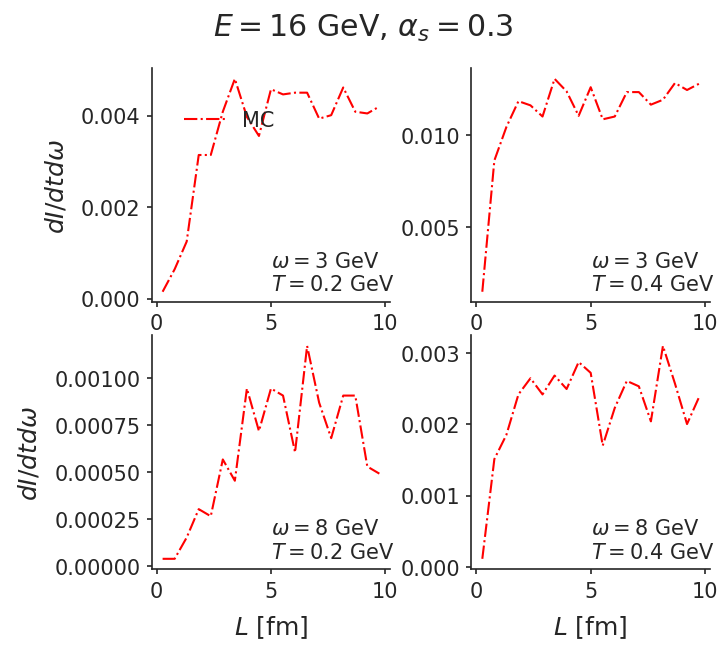
\includegraphics[width=\columnwidth]{spectrum_L.png}
\caption{Comparison of the path-length dependent energy-differential rate $dP/(dtd\omega)$ from the Monte-Carlo implementation using $\alpha_s = 0.3$ to the theoretical baseline calculation \cite{CaronHuot:2010bp}. The light quark energy is $16$ GeV.}
\label{fig:spectra-L-alphas=0.3}
\end{figure}

In Figure \ref{fig:spectra-L-alphas=0.3}, the spectrum in a finite medium is compared to the full calculations from \cite{CaronHuot:2010bp}.
Using $\alpha_s = 0.3$, we have calculated the $L$-dependent gluon radiation rate of a 16 GeV quark.
The medium temperature of the left and the right columns are 0.2 GeV and 0.4 GeV respectively.
Top and bottom rows show the differential rates for the emitting gluon with $\omega = 3$ GeV and $\omega = 8$ GeV \footnote{to facilitate our analysis, we have selected events within a finite range $\omega\pm 0.5$ GeV}.
The radiation spectrum is recovered to a similar level of accuracy as in the infinite medium case.

\subsection{Results in an expanding medium}
\begin{figure}
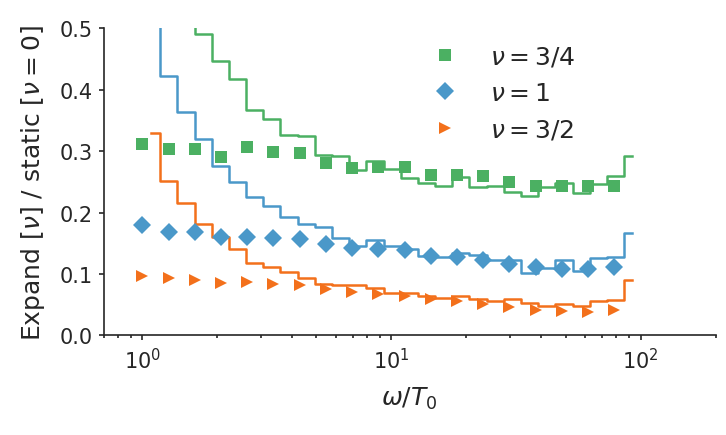
\includegraphics[width=\columnwidth]{spectrum_Bjorken.png}
\caption{The top frame shows the gluon radiation spectrum calculated with the the BDMPS formula (symbols) and Monte-Carlo simulations (lines) in a static medium ($\nu=1/2$), a slowly expanding medium ($\nu=5/7$) and a Bjorken expanding medium ($\nu\rightarrow 1$). In the bottom frame, we compute ratios of the analytic results and simulations between expanding cases and the static case. The parameters chosen are $\alpha_s=0.3$, $\tau_0 = 0.2$ fm/$c$, $L = 19.8$ fm/$c$, $T_0 = 1$ GeV.}
\label{fig:Bjorken-BDMPS}
\end{figure}

Next, we shall consider an expanding medium with a power law fall-off for the temperature: 
\begin{eqnarray}
T^3 = T_0^3\left(\frac{\tau_0}{\tau}\right)^{2-1/\nu}
\end{eqnarray}
The authors of \cite{Baier:1998yf} have calculated the radiation spectrum using the multiple-soft scattering approximation as,
\begin{eqnarray}
\frac{dP}{dx} &=& \frac{\alpha_s}{2\pi}P_{q\rightarrow qg}(x)\mathfrak{Re}\int_{\tau_0}^{\tau_0+L}\frac{dt_f}{t_f}\int_{\tau_0}^{t_f}\frac{dt_i}{t_i} \frac{1}{\nu^2}\\
\nonumber
&& \left.\left[ I_{\nu-1}(z_i)K_{\nu-1}(z_f)-I_{\nu-1}(z_f)K_{\nu-1}(z_i)\right]^{-2}\right|_{\omega}^{\omega=\infty},\\
z_{i,f} &=& 2i\nu \sqrt{\frac{\hat{q}_g(1-x+C_F/C_A x^2)}{2(1-x)\omega}} \tau_0 \left( \frac{t_{i,f}}{\tau_0}\right) ^{1/2\nu}
\end{eqnarray}
For $\nu=0.5$, this expression reduces to the static BDMPS result \cite{Baier:1996kr}. 
The Bjorken expansion $T \propto \tau^{-1/3}$ can be obtained by taking the limit $\nu \rightarrow 1$ \cite{PhysRevD.27.140}.
In an expanding medium, e.g. $\nu=1$, the transverse momentum broadening is,
\begin{equation}\label{eq:expanding-kt2}
\left\langle k_\perp^2\right\rangle \sim \int_{t_1}^{t_1+\tau_f
}\hat{q}(t)dt \sim \frac{t_1}{\tau_f}  \ln\left(1+\frac{\tau_f}{t_1}\right) \hat{q}(t_1)\tau_f
\end{equation}
So if the formation time is very short compared to the typical expansion time scale $d\ln(T)/d\tau \sim t_1$, the transverse broadening becomes $\left\langle k_\perp^2\right\rangle \sim \hat{q}(t_1)\tau_f$, which is the same as the one obtained in a static medium defined by the local temperature at $t_1$.
However, for large formation times, $\left\langle k_\perp^2\right\rangle$ becomes significantly smaller than the one determined using a local static medium.
The BDMPS calculation assumes multiple-soft scatterings, so we only use it in a medium thick enough that
\begin{eqnarray}\label{eq:BDMPS-requrement}
\omega_c \sim \left\langle k_\perp^2 \right\rangle L > E.
\end{eqnarray}

Moving toward a comparison in an expanding medium, we perform a calculation using only the diffusion and the diffusion induced radiation  processes with the ``modified rescattering" LPM implementation, since this setup allows us to use the same $\hat{q}_g$ in both the BDMPS formula and the Monte-Carlo calculation.
For simplicity, we choose $\hat{q}_g = m_D^2 C_A\alpha_s T$ without the logarithmic term, thus the $u$ factor in the acceptance is not required. 
The expansion starts at $\tau_0=0.2$ fm/$c$ with $T_0=1$ GeV. 
The evolution stops at $\tau = 20$ fm/$c$. 
In Table \ref{tab:expand}, we listed three cases $\nu = 1/2, 5/7, 1$ corresponding to a static medium, a slowly expanding medium and a medium with Bjorken flow respectively.
In the third column, the power of the falling temperature as function of proper time is calculated. The last column lists the temperature at the end of the evolution.
We verify that for a 100 GeV quark and $\alpha_s = 0.3$, the requirement of Equation \ref{eq:BDMPS-requrement} is satisfied.
The top frame of Figure \ref{fig:Bjorken-BDMPS} directly compares the spectra to the theory baseline and the bottom frame shows the ratio between the expanding cases over the static case. 
The Monte-Carlo calculation performs very well in the LPM region, reflecting the decrease of induced radiation due to the dropping of temperature.
One also notice that the level of agreement decreases with increasing expansion rate. 
This is not a surprise, because the Monte-Carlo procedure described here is still not a fully quantum treatment.
\begin{center}
\begin{table}[h]
\caption{Expanding medium setup}\label{tab:expand}
\begin{tabularx}{\columnwidth}{XXXX}
\hline
Type & $\nu$ & $(2-1/\nu)/3$ & $T_f$ [GeV]\\ 
\hline
Static & 1/2 & 0 & 1.0\\
\hline
Slow & 5/7 & 1/5 & 0.40\\
\hline
Bjorken & $\rightarrow 1$ & 1/3 & 0.22\\
\hline
\end{tabularx} 
\end{table}
\end{center}

\subsection{Implementing running coupling}
\begin{figure}
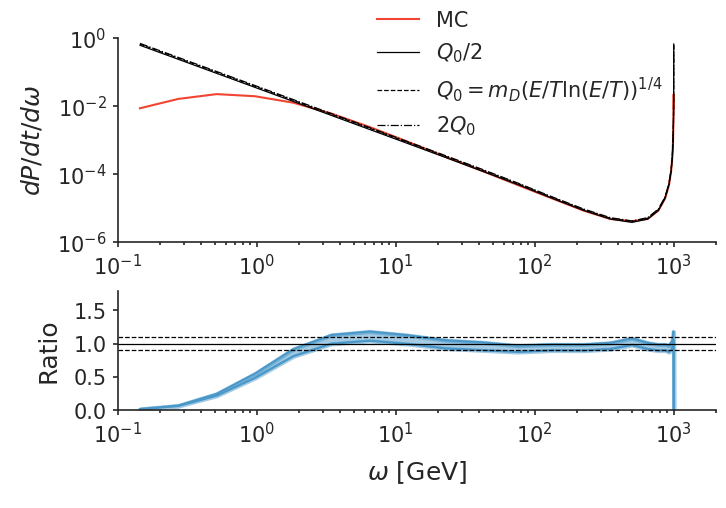
\includegraphics[width=\columnwidth]{running.png}
\caption{Comparison of the path-length dependent energy-differential rate $dP/(dtd\omega)$ from the Monte-Carlo implementation using $\alpha_s = 0.3$ to the theoretical baseline calculation \cite{CaronHuot:2010bp}. The light quark energy is $16$ GeV.}
\label{fig:spectra-L-alphas=0.3}
\end{figure}

This section focus on improving our model by introducing a running coupling constant and mass effects. 
However, due to their complexity, we did not found applicable theory baseline results to compare to.
As a result, the proposed methods in this section should be considered as tentative.

We replace the fixed coupling by a running coupling constant  following the prescription described in \cite{Arnold:2008zu}.
This involves two changes in the formula. 
For elastic scattering vertices, $\alpha_s^{\textrm{el}}$ is evaluated at the $t$-channel momentum transfer squared. 
This is already the feature of {\tt Lido}.
For splitting vertices,  $\alpha_s^{\textrm{rad}}$ should be evaluated at the final gluon transverse momenta squared,
\begin{eqnarray}\label{eq:kTn}
k_{\perp,n}^2 = \left(\vec{k}_{\perp,0}+\vec{q}_1+\cdots+\vec{q}_n\right)^2.
\end{eqnarray} 
In the {\tt Lido} model, the original scale used for $\alpha_s^{\textrm{rad}}$ is $k_{\perp,0}^2$ from the $2\rightarrow 3$ process.
Therefore, we modify the acceptance probability $p$ to
\begin{eqnarray}
p' = \min\left\{1, u\frac{\tilde{\lambda}}{\tau_f}\frac{\alpha_s(k_{\perp,n})}{\alpha_s(k_{\perp,0})}\right\}.
\end{eqnarray}
The order of magnitude of $k_{\perp,n}^2$ is $\sqrt{\hat{q}\omega}$ and it is about $\sqrt{\omega/T}$ times larger than $k_{\perp,0}^2$ for gluons in the LPM region, therefore the running coupling effect suppresses the spectrum by another factor of $\alpha_s(k_{\perp,n})/\alpha_s(k_{\perp,0})$.
In Figure \ref{fig:run}, we show three calculations in a static medium. The dotted lines, as references, uses a fixed coupling constant evaluated at a thermal scale $\alpha_s = \alpha_s(2\pi T)$ .
This scale is also the lowest scale cut-off for the running coupling constant in our model \footnote{please see Appendix \ref{app:alphas} for details. Note that this minimum scale is not required in the original work \cite{Arnold:2008zu} where all scales are assumed to be much greater than $\Lambda_{\textrm{QCD}}$.}.
The dash-dotted lines are running coupling calculations where the $\alpha_s^{\textrm{el}}$ is evaluated at $\hat{t}$ and the $\alpha_s^{\textrm{rad}}$ at $k_{T,0}$.
The dashed lines are also running coupling calculations but evaluate $\alpha_s^{\textrm{rad}}$ at $k_{\perp,n}$ through the modified acceptance $p'$.
The running coupling effect results in a reduction of the energy loss compared to the fixed coupling references.

\subsection{Outlook for mass effect}
Finally, we include quark mass dependencies in our calculation in order to expand our LPM treatment to heavy quarks. These include the massive particle kinematics, a substitution in the formation time,
\begin{eqnarray}
(1-x)m_\infty^2 \rightarrow x^2M^2 + (1-x)m_\infty^2
\end{eqnarray}
and the so-called ``dead-cone" effect that suppresses collinear radiations with angles $\theta \sim k_\perp/k < M/E$. 
The massive version of the $2\rightarrow3$ improved Gunion-Bertsch matrix-element has been derived in \cite{Uphoff:2014hza}.
If we simply replace the matrix-element with the massive one, the dead cone suppression involves the factor,
\begin{eqnarray}
\frac{k_{\perp,0}^2}{k_{\perp,0}^2+x^2M^2}
\end{eqnarray}
However, because rescatterings continue to increase the average $k_{\perp}^2$ , the factor is different by the time the gluon is formed,
\begin{eqnarray}
\frac{k_{\perp,n}^2}{k_{\perp,n}^2+x^2M^2}.
\end{eqnarray}
The solution is to use the $2\rightarrow3$ matrix-element without mass effect to generate pre-formed gluons, while implementing the dead-cone suppression by adding another factor to the acceptance,
\begin{eqnarray}
p'' = \min\left\{1, u\frac{\tilde{\lambda}}{\tau_f}\frac{\alpha_s(k_{\perp,n})}{\alpha_s(k_{\perp,0})} \left[\frac{k_{\perp,n}^2}{k_{\perp,n}^2+x^2 M^2}\right]^4\right\}.
\end{eqnarray}
On the left of Figure \ref{fig:mass}, the scaled energy loss rate in an infinite medium is extracted from simulations for light (massless), charm ($M=1.3$ GeV) and bottom ($M=4.2$ GeV) quarks. 
On the right, it is the energy loss fraction at a fixed path-length $L=5$ fm.
In both cases, the mass introduces the energy loss ordering, $\Delta E_{\textrm{light}} > \Delta E_c > \Delta E_b$ and the differences decrease at higher energy.

%\begin{figure*}
%\includegraphics[width=\textwidth]{raa_mclpm.pdf}
%\caption{This figure shows what is predicted for D-meson observables at the leading order level considering running coupling and mass effect. The only parameter is the minimum scale in the running $\alpha_s(\max\{Q,\mu\})$. The solid lines use $\mu = 2\pi T$ and the dashed lines use $\mu=\pi T$}
%\end{figure*}


\section{Summary and outlook}\label{section:summary}
We have studied three different Monte-Carlo implementations of the LPM suppression of jet energy-loss and have compared them to a theory baseline.
We have shown that the ``modified rescattering" approach reproduces the coupling constant, temperature, parton energy and path-length dependences of the theoretical baselines for both infinite- and thin-medium limits.
The overall level of agreement between the simulated radiation spectrum and theory is promising given the simplicity and limits of a Monte-Carlo procedure. Tentative running coupling and dead-cone effect dependencies have also implemented.
This work allows us to reduce the theory uncertainty introduced in the numerical implementation of the perturbative QCD transport of hard partons inside a quark-gluon plasma, which is instrumental for performing an unambiguous examination of theory assumptions and a more meaningful phenomenological extraction of jet and heavy quark transport properties in a model-to-data comparison.
Moreover, a Monte-Carlo generator that is tuned to match leading order theory calculation will serve as a promising starting point to implement next-to-leading-order effects in the phenomenology model.


\begin{acknowledgments}
SAB, WK and YX are supported by the U.S. Department of Energy Grant no. DE-FG02-05ER41367. WK is also supported by NSF grant OAC-1550225.
WK would like to thank Florian Senzel, Jean-Francois Paquet and Yacine Mehtar-Tani for helpful discussions.
\end{acknowledgments}

\begin{appendices}
\section{Running coupling constant}\label{app:alphas}
The leading order running couplings constant with three quark flavors is
\begin{eqnarray}
\alpha_s(Q) = \frac{4\pi}{9\log(Q^2/\Lambda_{\textrm{QCD}}^2)},
\end{eqnarray}
and $\Lambda_{\textrm{QCD}} = 0.2$ GeV. In a medium, we require that the scale of a process cannot be arbitrarily small compared to the temperature. The resulting $Q$ is cut off at a medium scale defined by $\mu\pi T$ ($\mu=2$ by default) and $\alpha_s(Q) = \alpha_s(\max\{Q,\mu\pi T\})$. We treat $\mu$ as a parameter of the model. It is also a major source of uncertainty in the predictions. In fact for a typical $T=0.3$ GeV, $\alpha_s(\pi T \sim 4\pi T)$ varies from 0.45 to 0.24.

\begin{figure}
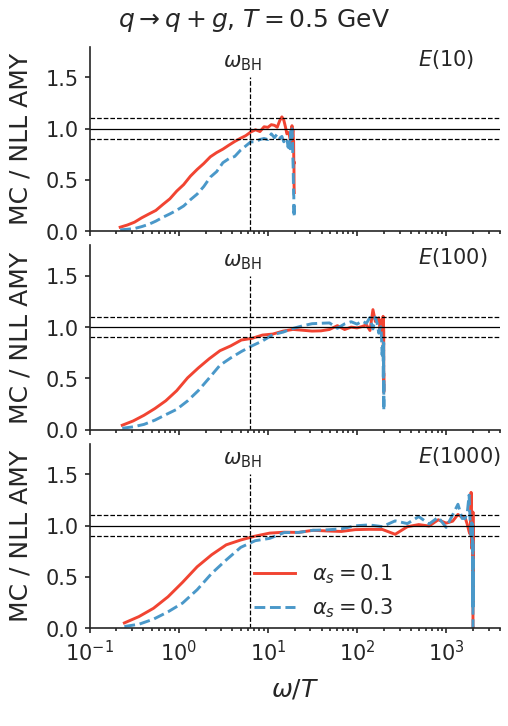
\includegraphics[width=\columnwidth]{spectrum_E_q2qg.png}
\caption{Ratios of Monte-Carlo calculated gluon emission spectra to the AMY NLL spectra (gray bands) and to the Gunion-Bertsch incoherent spectra (blue lines), using $\alpha_s = 0.1$. The quark energies are $E$ is 10, 50, 100, and 500 GeV as indicated by the rightmost vertical dashed lines in each subplot. The horizontal dashed lines denote $\pm 10\%$ deviation from unity.}
\label{fig:spectra-alphas=0.1}
\end{figure}

\begin{figure}
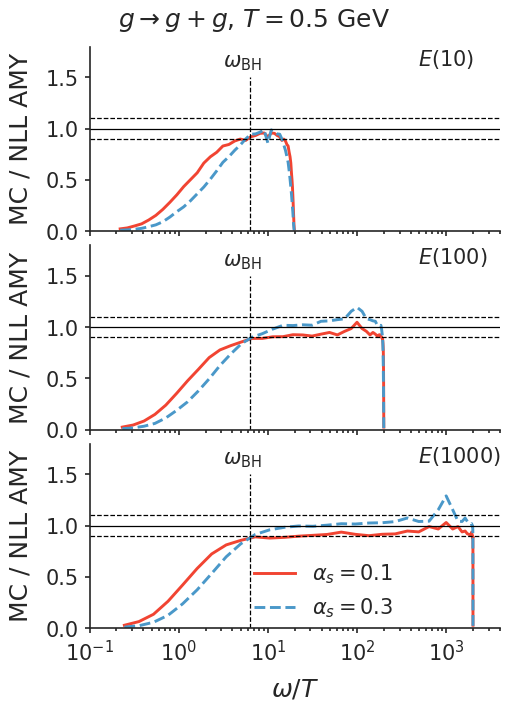
\includegraphics[width=\columnwidth]{spectrum_E_g2gg.png}
\caption{Ratios of Monte-Carlo calculated gluon emission spectra to the AMY NLL spectra (gray bands) and to the Gunion-Bertsch incoherent spectra (blue lines), using $\alpha_s = 0.1$. The quark energies are $E$ is 10, 50, 100, and 500 GeV as indicated by the rightmost vertical dashed lines in each subplot. The horizontal dashed lines denote $\pm 10\%$ deviation from unity.}
\label{fig:spectra-alphas=0.1}
\end{figure}

\begin{figure}
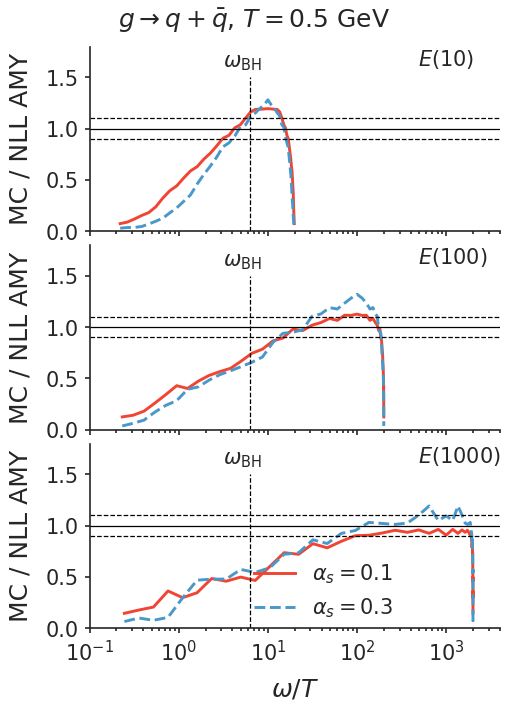
\includegraphics[width=\columnwidth]{spectrum_E_g2qqbar.png}
\caption{Ratios of Monte-Carlo calculated gluon emission spectra to the AMY NLL spectra (gray bands) and to the Gunion-Bertsch incoherent spectra (blue lines), using $\alpha_s = 0.1$. The quark energies are $E$ is 10, 50, 100, and 500 GeV as indicated by the rightmost vertical dashed lines in each subplot. The horizontal dashed lines denote $\pm 10\%$ deviation from unity.}
\label{fig:spectra-alphas=0.1}
\end{figure}

\section{Energy and coupling constant dependence of radiation spectra}\label{app:tune-spectrum}
It is important to be aware of the known discrepancies between the Monte-Carlo implementation and the theory baseline, particularly if one investigates an observable that is sensitive to the details of the radiation spectra. 
In this appendix, we provide comparisons of radiation spectra at different values of energy and coupling constant for the reader's references.
Figure \ref{fig:spectra-alphas=0.1} and Figure \ref{fig:spectra-alphas=0.3} shows calculation using $\alpha_s = 0.1$ and $0.3$.
Within in each figure, different subplots vary the quark energy.
The gray bands are the ratios between the simulations and the AMY-NLL results (plotted for $\pi T < \omega < E$) and the blue lines are the ratios between the full simulations and the incoherent simulations (the Gunion-Bertsch rate, plotted for $0.1$ GeV $< \omega < 4\pi T $).
We notice that there are residual systematic discrepancies, but the overall difference is controlled within $\pm 15\%$ for the coupling constants, temperatures and energies under consideration.

\end{appendices}
\bibliography{mclpm} 
\end{document}
